\documentclass{article}
\usepackage{graphicx} % Required for inserting images

\title{PELEE Statistical Update}
\author{Alexandra Trettin}
\date{October 2023}

\begin{document}

\maketitle

\section{Introduction}

The PELEE Statistical Update is an upgraded version of the PELEE analysis where we add runs 4 and 5. In addition to the addition of more statistics, some improvements to the event selection, signal modelling and treatment of systematics have also been made that are documented here. 

\subsection{Goals of this analysis}
(Giuseppe, work in progress.)

Goal of this analysis is to perform a statistical update of the first pionless eLEE analysis, thus checking with a larger dataset the stability of the results and comparing the data to a signal model that relies less on assumptions about the physics process leading to the excess in MiniBooNE.

Therefore, updates to the analysis are primarily of statistical nature, either in terms of the amount of data included, or in terms of the statistical procedures used to extract the result:
\begin{itemize}
    \item Include the full MicroBooNE BNB data, from run1 to run5.
    \item Update the signal model of the MiniBooNE excess, now based on the electron kinematics.
    \item Update the statistical treatment of the cosmic background (estimated with triggered beam-off, "EXT", events)
    \item Explore potential updates to other statistical procedures, such as correlations for detector variations, and the constraint selection.
\end{itemize}
The only selection update we consider in this update is the usage of the CRT veto in the nue selection for run3-5. This selection was already used in the numu selection (for constraint) in the first round of the analysis and it makes sense to use it also for the nue selection given that all the additional data include the CRT detector.

Further updates to the reconstruction and to the selection will be included in the final version of the analysis, which is planned for 2025.

\section{Event Selection}
focus on changes with respect to the previous selection
(Kate + Sophie)

\subsection{Selection validation}
\label{sec:selvalid}
Describe validation of run 4 and 5 selection

Technical verification of the framework (Chris)

Show consistency across runs
Compare variables across runs, data/MC plots 
For example, runs 123 compared to run 4 and 5 separately

Check things like consistency of calorimetry, rate of cosmics, inputs into the BDT
Fan's plots for run 4 and 5 validation (Fan)

\newpage
\section{Sidebands}
\label{sec:sidebands}
Consistency checks in each sideband
0p and Np variation of two-shower sideband, inverted BDT sideband
Consistency at different selection stages:
preselection, loose selection, full selection
see Chapter 11(?) of the previous note

\section{Signal model}
Describe Fan's signal model (Fan)

\section{Systematics and expected sensitivity}
(outline by David)

\subsection{Systematics: unchanged}What is the same as Run 1-2-3 analysis: few sentences + reference past note.
\subsection{Systematics: What's new}
\subsubsection{GENIE FSI bug-fix} A few validation plots, e.g. Chris' validation work of GENIE weights.
\subsubsection{EXT smoothing} (Alex)
\subsubsection{DetVar systematics} Are we assuming Run123 detvars for Run 1-5? Probably true for first sensitivites. \\
Include a table which lists MC stats available on DetVar samples.
\subsubsection{Signal model systematics}

\subsection{systematics summary}

The total systematics error budget is shown in the table of Fig.~\ref{fig:systematicsbudget}.

\begin{center}
\begin{figure}[h]
    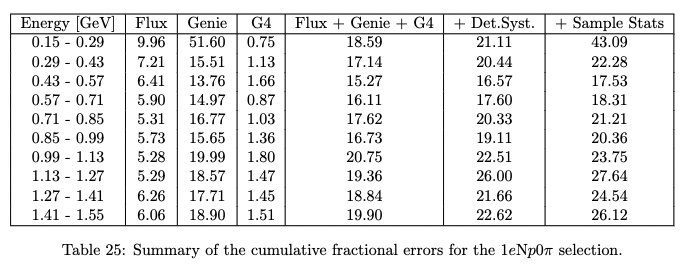
\includegraphics[width=1.00\textwidth]{technote/images/systematicsbudget.png}
    \caption{\label{fig:systematicsbudget} Enu spectrum before/after constraint.}
\end{figure}
\end{center}

\newpage
\subsection{Constraints}
Describe briefly, refer to older analysis.

Show spectrum of nues before and after constraint. See Fig.~\ref{fig:constraint}.

\begin{center}
\begin{figure}[h]
    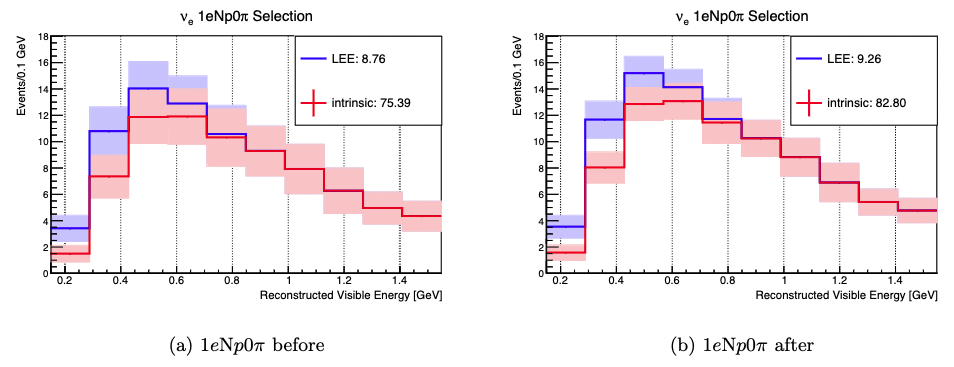
\includegraphics[width=1.00\textwidth]{technote/images/constraint.png}
    \caption{\label{fig:constraint} Enu spectrum before/after constraint.}
\end{figure}
\end{center}

Show quantitative predicted events and uncertainty (including reduction in uncertainty) before/after constraint. See Table of Fig.~\ref{fig:constrainttable}.

\begin{center}
\begin{figure}
    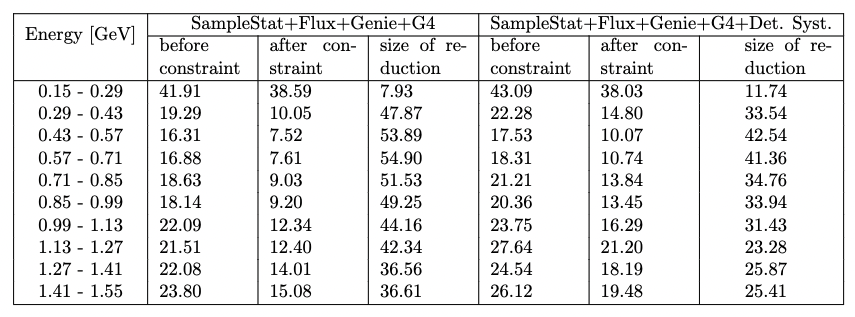
\includegraphics[width=1.00\textwidth]{technote/images/constrainttable.png}
    \caption{\label{fig:constraint} Impact of constraint.}
\end{figure}
\end{center}

Potentially think of new ideas here

\newpage
\subsection{Sensitivity}
\label{sec:sensitivity}

\subsubsection{Simple Hypothesis Test}

Distribution of test statistic for backgronud-only and signal models, with extracted median sensitivity. See. Fig.~\ref{fig:simplehypothesis}.

\begin{center}
\begin{figure}[h]
    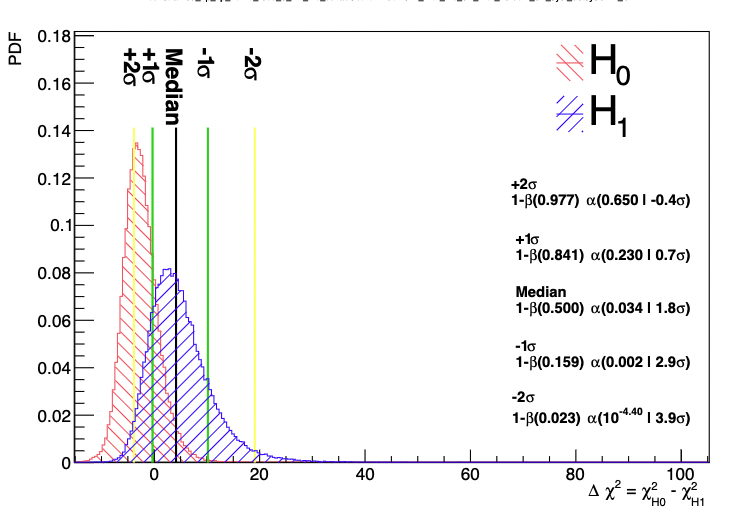
\includegraphics[width=1.00\textwidth]{technote/images/simplehypothesis.png}
    \caption{\label{fig:simplehypothesis} Impact of constraint.}
\end{figure}
\end{center}

Fig.~\ref{fig:simplehypothesisresults} shows the expected sensitivity for the simple hypothesis test.

\begin{center}
\begin{figure}[h]
    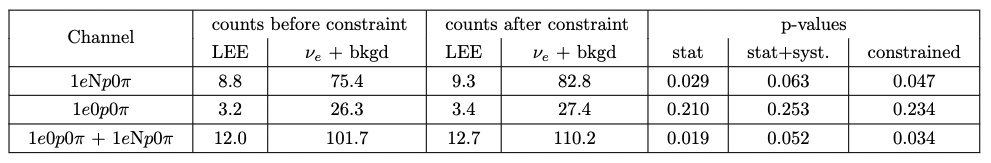
\includegraphics[width=1.00\textwidth]{technote/images/simplehypothesisresults.png}
    \caption{\label{fig:simplehypothesisresults} Impact of constraint.}
\end{figure}
\end{center}

\newpage
\subsubsection{Signal strength fit}

The signal strength sensitivity results are shown in Fig.~\ref{fig:signalstrengthsensitivity}.
\begin{center}
\begin{figure}[h]
    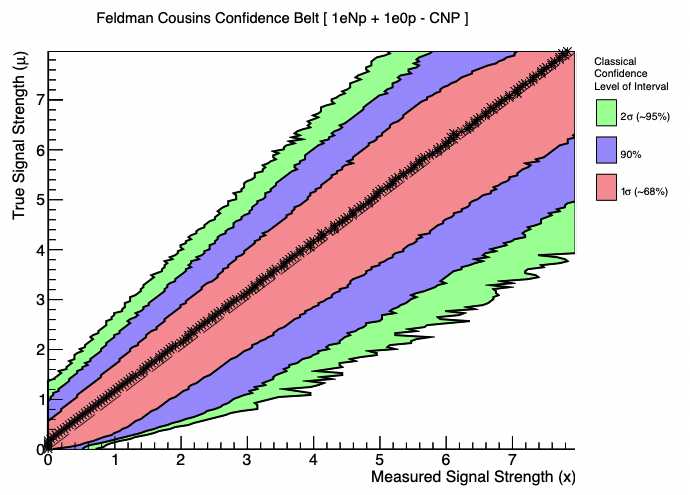
\includegraphics[width=1.00\textwidth]{technote/images/signalstrengthsensitivity.png}
    \caption{\label{fig:signalstrengthsensitivity} Impact of constraint.}
\end{figure}
\end{center}

\newpage
\subsubsection{Validation of sensitivity vs. SBNFit benchmark}

\newpage
\section{Unblinding strategy}
(Giuseppe, work in progress)

\begin{itemize}
    \item Validate the selection variables in the new run periods (see Sec.~\ref{sec:selvalid}).
    \item Verify the selection makes sense on the small open datasets.
    \item Study sidebands (2-shower selection, events failing the BDT cut, events with higher-energy electrons) along the lines of studies performed for the first result (see Sec.~\ref{sec:sidebands}).
    \item Do we want to consider updating the constraint procedure in case of specific tension in sidebands? For instance, if the 2-shower sideband shows a trend vs the pi0 energy, include it in the constraint? Well, we already know it, but with more data the effect may become more significant.
    \item Once results in the sidebands are understood, in case of no pending issues and when all statistical procedures are settled (see Sec.~\ref{sec:sensitivity}), we'll proceed to unblinding the signal region. 
    \item List here the plots that will be part of the "result" and the additional validation checks we'll do post-unblinding.
    \item Consider discuss a "flow chart" of the ublinding process, and what actions are taken depending on the outcome of the analysis.
\end{itemize}

\end{document}